% --------------------------------------------------------------------------------

\begin{exercise}[Sum and average]

Let $X$ be a random variable with $\mathcal N(5, 2^2)$.
Let $X_1, X_2, \dots X_{50}$ be independent identically distributed copies of $X$.
Let $S$ be their sum and $\bar X$ their average, i.e.

\begin{align*}
    S = X_1 + \cdots X_{50}
    \quad
    \text{and}
    \quad
    \bar X = \frac{1}{50} (X_1 + \cdots + X_{50}).
\end{align*}

\begin{enumerate}[label = (\alph*)]

    \item Plot the density and the distribution function for $X$ using R.

    \item What are the expectation and the standard deviation of $S$ and of $\bar X$?

    \item Generate a sample of $50$ numbers from $\mathcal N(5, 2^2)$.
    Plot the histogram for ths sample.
    Do the same for a sample of $500$ numbers from $\mathcal N(5, 2^2)$.

\end{enumerate}

\end{exercise}

% --------------------------------------------------------------------------------

\begin{solution}

\phantom{}

\begin{enumerate}[label = (\alph*)]

    \item \phantom{}
    
    \lstinputlisting{4.4.a.r}

    \begin{figure}[H]
        \centering
        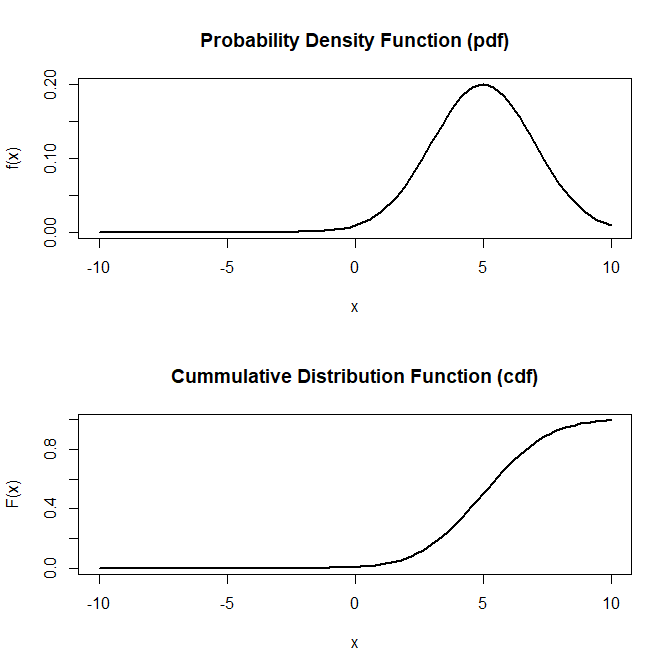
\includegraphics[width = 0.75 \textwidth]{4.4.a.png}
        \caption{}
        \label{}
    \end{figure}

    \item $S \sim \mathcal N(50 \cdot 5, 50 \cdot 2^2)$, $\bar X \sim \mathcal N(5, \frac{2^2}{50})$

    \item \phantom{}

    \lstinputlisting{4.4.c.r}

    \begin{figure}[H]
        \centering
        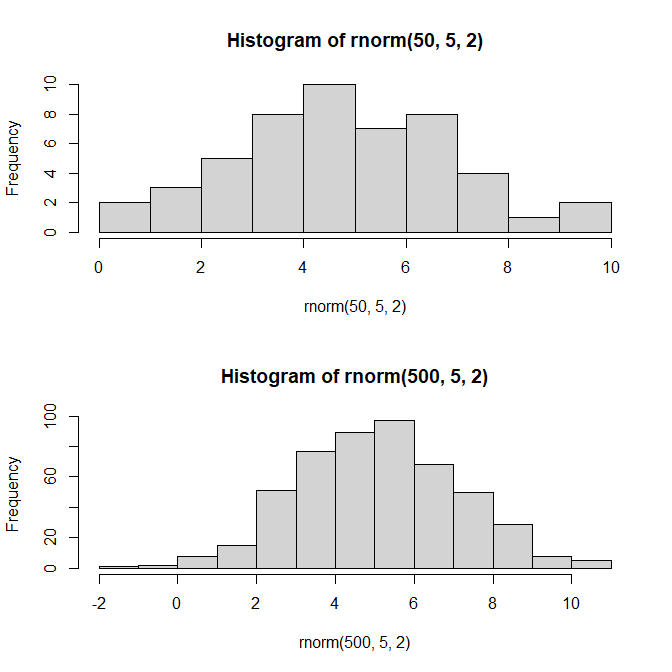
\includegraphics[width = 0.75 \textwidth]{4.4.c.png}
        \caption{}
        \label{}
    \end{figure}

\end{enumerate}

\end{solution}

% --------------------------------------------------------------------------------
